% -*- mode: fundamental -*-

% ****************************************************************

\chapter{Pending}

\markboth{Ch \arabic{chapter}: Pending (DRAFT)}{\copyrightnotice}

\setcounter{page}{1}
% \renewcommand{\thepage}{\arabic{page}}
\renewcommand{\thepage}{\arabic{chapter}-\arabic{page}}

\label{ch_Pending}

% ****************************************************************

This is a place-holder chapter with a TODO list of pending possible
topics to be written.

\begin{figure}[htbp]
  \centerline{\includegraphics[width=6in,angle=0]{ch030_RISCV_Design_Space/Figures/Fig_Simple_Instr_Exec}}
  \caption{\label{Fig_Pending_Simple_Instr_Exec}Simple interpretation of RISC-V instructions (same as Fig.~\ref{Fig_Simple_Instr_Exec})}
\end{figure}

\hdivider

% ****************************************************************

\section{Drum: Traps and Interrupts, and basic CSRs}

Note: These (implementation-independent) explanations may already be
done in Chapter~\ref{ch_ISA} on the RISC-V ISA:

\begin{tightlist}
  \item Explanation of illegal instruction traps
  \item Explanation of Fetch memory-access traps
  \item Explanation of LOAD/STORE/AMO memory-access traps
\end{tightlist}

Overview of how a trap is handled, using minimal set of CSRs (Control
and Status Registers): MCAUSE, MTVAL, MEPC, MTVEC, MCAUSE, MRET.

CSR register file and CSRRxx instructions to access them.

CSR (Control Status Registers)

% ================================================================

\subsection{Drum: Interrupts}

Interrupts in Drum:
\begin{tightlist}
  \item General concepts: MIP and MIE registers, MSTATUS.interrupt-enable-bit.

  \item Interrupts are initially disabled using the
        MSTATUS.interrupt-enable bit immediately; CSRxx can be used to
        re-enable.

  \item Interrupts are handled just like traps; the only question is:
        when to check for interrupts and respond.

  \item How does MIE bit return to 0?

\end{tightlist}

\hdivider

% ****************************************************************

\section{Fife: pipelined execution}

Fife: Basic concepts of pipelined execution of instructions, {\ie}
pipelined implementation of the abstract algorithm of
Figure~\ref{Fig_Pending_Simple_Instr_Exec}.

Fife: parallel execution pipes for ``Execute'' steps in
Figure~\ref{Fig_Pending_Simple_Instr_Exec}

\begin{tightlist}

  \item Dispatching to different pipes after Register-Read

  \item Results from ``Execute'' pipes may be ready in different order from dispatch.

  \item   Tagging each pipe so ``Retire'' stage can retire in-order
\end{tightlist}


% ================================================================

\subsection{PC-prediction (control speculation)}

PC-prediction
\begin{itemize}
  \item The need for at least a minimal PC-prediction in Fetch stage:
        for many instructions, next-PC may not be known until deep in
        the pipeline; if so, what should Fetch do in the meantime?

    \begin{itemize}

      \item for conditional-branches (BRANCH) and jumps (JAL and
            JALR), next-PC is not known until ``Control'' step of the
            pipe.  What should Fetch do in the meantime?

      \item If there is a trap, next-PC changes from the normal next-PC.

        \begin{itemize}

          \item An instruction-fetch may trap, which we will discover
                only in memory-response arriving at the Decode stage

          \item The decode stage may find that the fetched
                ``instruction'' is not a legal instruction.  This
                causes a trap.

          \item An instruction may trap in the Execute stage ({\eg},
                LOAD/STORE/AMO may trap in memory access)

        \end{itemize}
    \end{itemize}

  \item The simplest predictor: PC+4

  \item Handling mispredictions: epochs, carrying epochs on
        instructions, discarding wrong-epoch.  How many epochs are
        needed?

  \item More advanced predictors
\end{itemize}

% ================================================================

\subsection{Register read/write hazards in Fife}

Scoreboards, scoreboard management, stalling-while-scoreboard busy.

Brief discussion of bypassing?

% ================================================================

\subsection{Speculative vs. non-speculative memory ops}

``Execute Memory Ops'' stage is always speculative (because of
mispredictions, and because older instructions in other pipes may
trap).

\begin{tightlist}
  \item Need for store-buffer and final commit/discard from Retire-stage
  \item Mem-system performs store only in store-buffer
  \item Retire stage sends commit/discard message to store-buffer.
        Discuss: do we need 'discard' messages, or are 'commit' messages enough?
\end{tightlist}

What about MMIO?

\begin{tightlist}
  \item LOADs may have side-effects
  \item LOADs may not be idempotent
  \item STOREs may have side-effects in addition to value stored
  \item LOAD may not return most-recently stored value
\end{tightlist}

So, these cannot be done speculatively, {\ie} in ``Execute Memory
Ops'' stage.

\begin{tightlist}

  \item 'Execute Memory ops' stage defers the request by sending it
    back as another kind of 'response'

  \item Retire step performs it once we know it is non-speculative.
\end{tightlist}

% ================================================================

\subsection{Fife: CSRs}

\begin{tightlist}
\item CSRRxx are read-modify-write operations
\item CSRRxx access may not be memory-like (side-effecting reads, read
      may not return last written value,
\item ... (a bit like MMIO issues)
\end{tightlist}
Hard to pipeline, so execute in Retire stage, as FSM.

CSRRxx instructions should be rare, so FSM exec does not affect overall performance.

% ================================================================

\subsection{Fife: Interrupts}

Sample for interrupts in Retire stage, fix up CSRs and and redirect.

Retire stage already has infra for CSR update and redirection, so this
is a small incremental change.

% ================================================================

\subsection{Measurements for Performance Analysis}

MTIME, MCYCLE, MINSTRET

``hpmcounter'' CSRs for other events.

\hdivider \\
\hdivider

% ****************************************************************
% ****************************************************************
% ****************************************************************

\section{Advanced topics, possibly in a separate ``Book 2''}

Goal: Linux capability, better performance.

% ================================================================

\subsection{Advanced branch prediction}

Is a form of online machine-learning.

Branch instruction hints.

Branch-Target buffers (BTBs)

Return-Address Stacks (RASs)

Hysteresis in prediction.

% ================================================================

\subsection{Caches}

Separate I- and D-caches.

FENCE.I: for ``manual'' I- and D-Mem coherence.

FENCE: flushing caches for for devices.

Cache-coherence.

% ================================================================

\subsection{Compressed instructions}

Implementation: wholly in Decode stage.  Common shared between Fife and Drum.

Affect of compressed instructions on Fetch.

Affect of compressed instructions on PC-prediction.

Affect of non-32-bit alignment of compressed instructions.

% ================================================================

\subsection{AMO operations}

Note: These (implementation-independent) explanations may already be
done in Chapter~\ref{ch_ISA} on the RISC-V ISA:

\begin{itemize}
  \item Explanation of LR and SC instructions
  \item Explanation of AMOxxx instructions
  \item Implementation in the memory system
\end{itemize}

% ================================================================

\subsection{Multiple Privilege levels}

Machine, Supervisor, User

Interrupt/trap delegation.

Hypervisor

% ================================================================

\subsection{Memory Protection with PMPs}

Page Tables, TLBs

% ================================================================

\subsection{Virtual Memory}

Page Tables, TLBs

% ================================================================

\subsection{RISC-V ISA Formal Specification}

Sail model

% ****************************************************************
